\pdfoutput=1

\documentclass[11pt,landscape]{article}


\setlength{\oddsidemargin}{0in}		% default=0in
\setlength{\textwidth}{9in}		% default=9in

\setlength{\topmargin}{-1in}		% default=0.20in
\setlength{\headsep}{0.25in}		% default=0.35in

\usepackage{graphicx}
 \usepackage{eurosym}
 \usepackage{hyperref}
 \usepackage[3D]{movie15}
\usepackage{caption}

\begin{document}

\thispagestyle{empty}

\begin{figure*}[htb!]
\centerline{\includemovie[poster, toolbar, 3Dc2c = 0 0 1, 3Droo= 70, 3Droll = 90, 3Dlights= CAD, 3Dbg = 50 50 50, label=dice, text={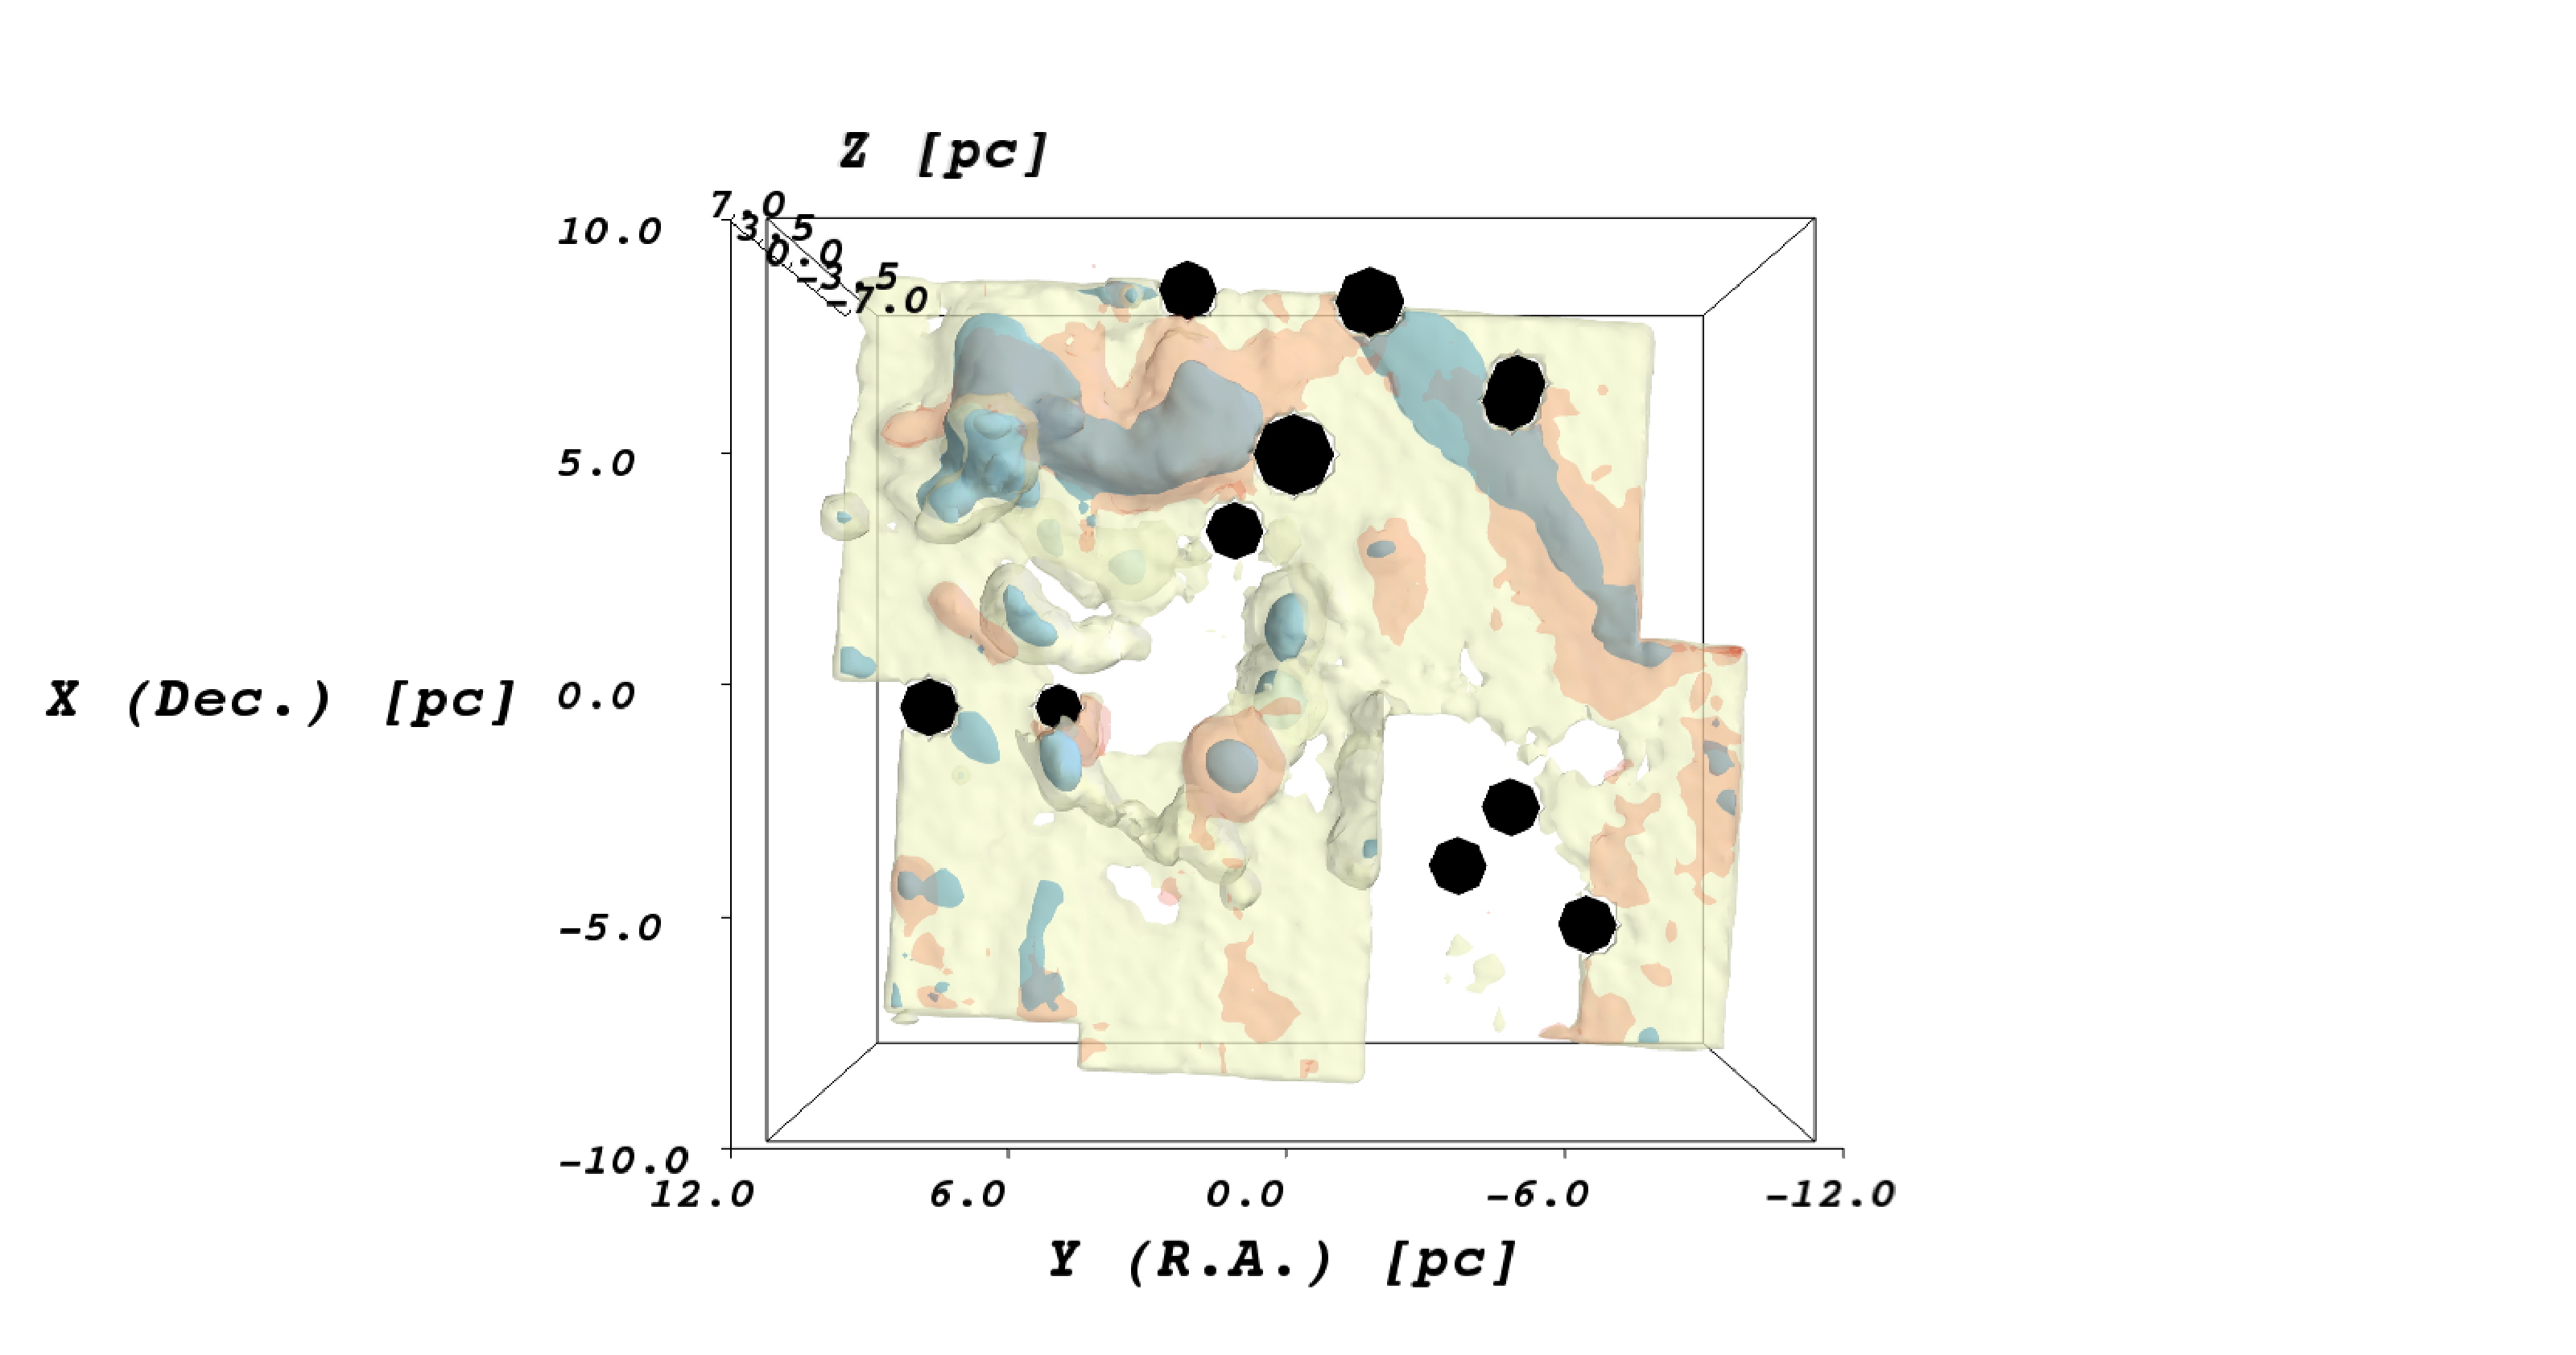
\includegraphics[scale=0.43]{./Vogt+Shingles.eps}}]{1.0\linewidth}{ 0.6\linewidth}{./Vogt+Shingles.u3d}}
\caption*{3D projection of the oxygen-rich ejecta in the supernova remnant N132D, as seen from the Earth. Oxygen emission is in blue and yellow, hydrogen in red, and chopped-off foreground stars are marked by black spheres. Oxygen-rich knots that were expelled from the outer layers of the progenitor star during the supernova explosion are identified as the hydrogen-free clumps. The axes are in parsec, where 1 pc $\cong$ 3.1$\times10^{13}$ km . The ejecta form a distorted ring structure, best revealed in an animation of this 3D map. \textbf{In the electronic version of this figure, an interactive 3D model can be loaded by clicking on the image} (Adobe Acrobat Reader v.9.0 or above is required). \textbf{In addition, an animation of the 3D map is stored in an \emph{augmented reality layer} accessible by snapping a picture of this figure with a smartphone and using the Layar app}. For more details, see Vogt and Dopita, Ap\&SS 311, 521 (2011) and Vogt and Shingles, Ap\&SS (2013, submitted), or email \href{mailto:fvogt@mso.anu.edu.au}{\nolinkurl{fvogt@mso.anu.edu.au}}.}\label{fig:n132d}
\end{figure*}

\end{document}
